\section{GenericRC Class Reference}
\label{classGenericRC}\index{GenericRC@{GenericRC}}
{\tt \#include $<$genericRC.h$>$}

Collaboration diagram for GenericRC:\nopagebreak
\begin{figure}[H]
\begin{center}
\leavevmode
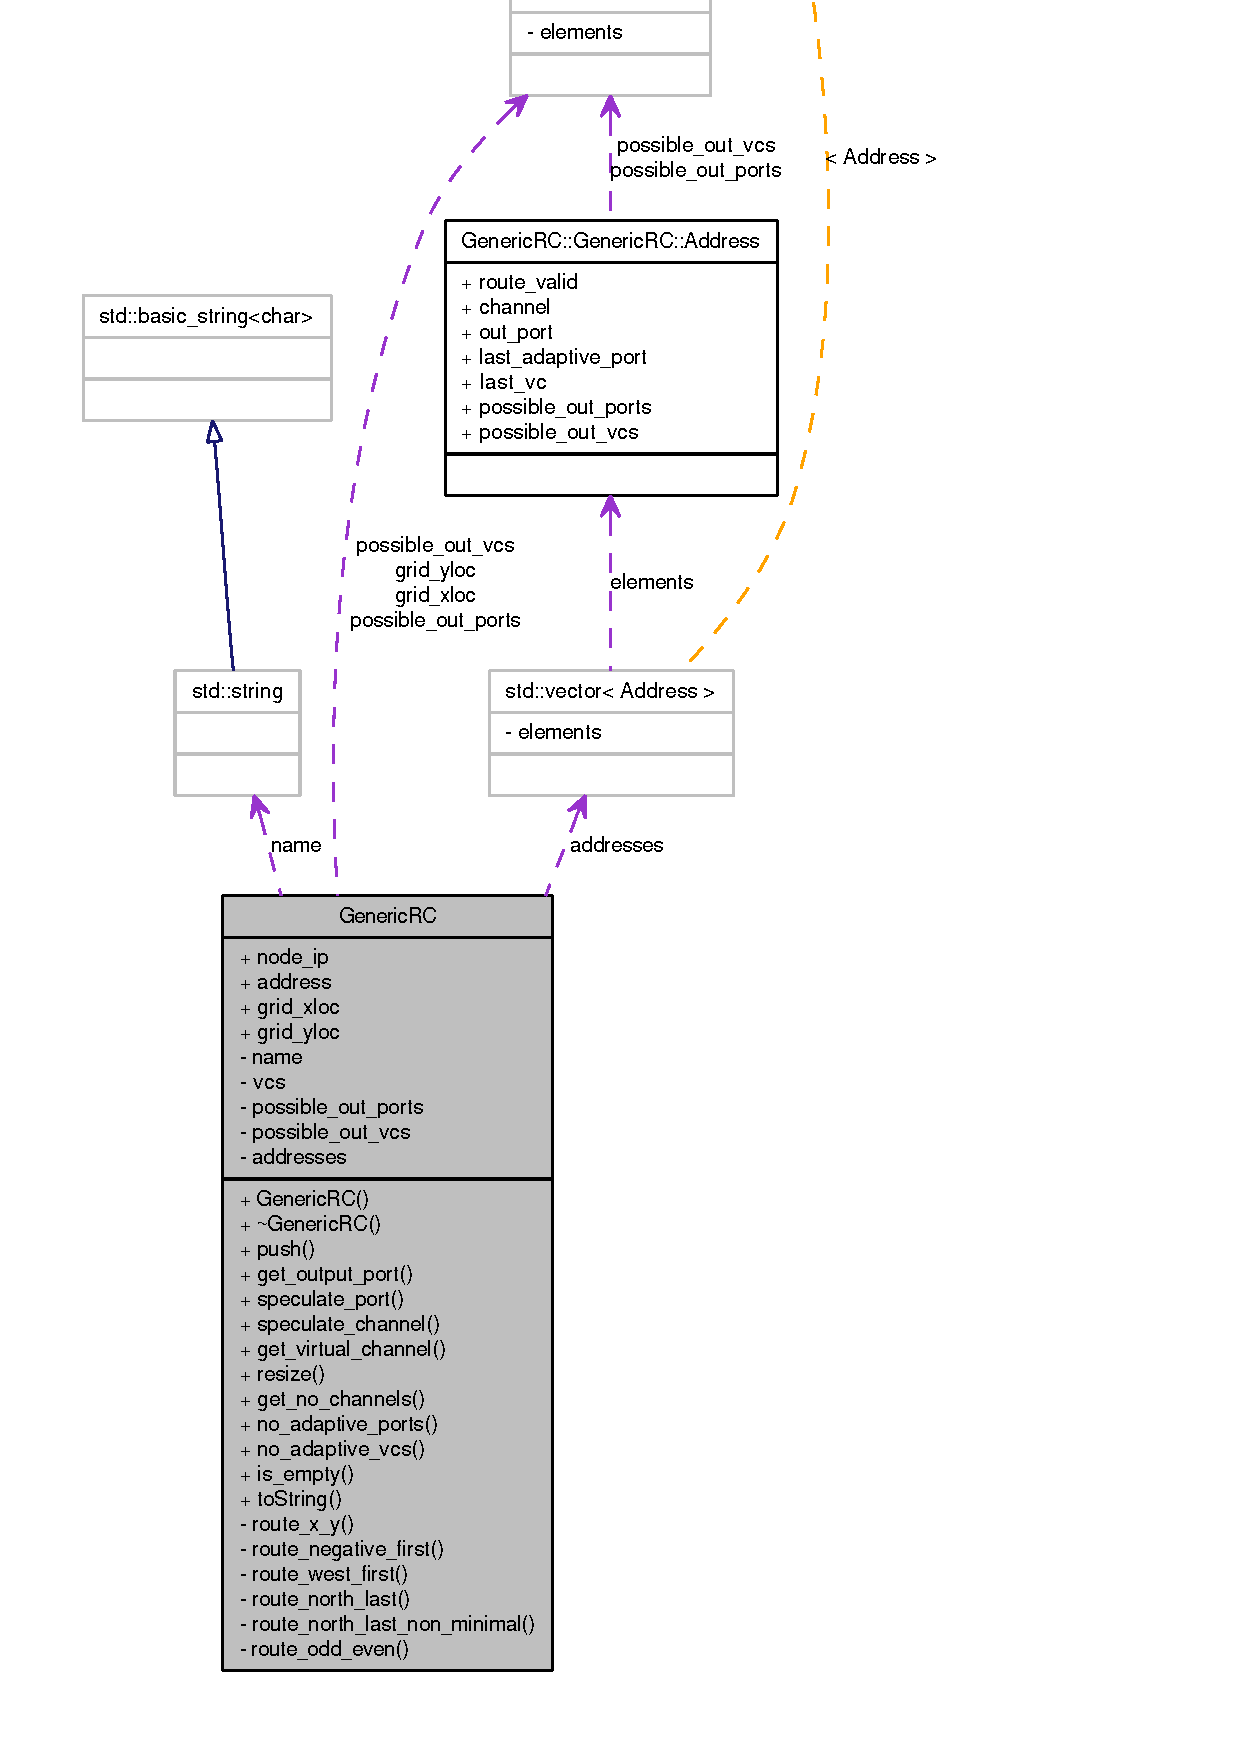
\includegraphics[width=400pt]{classGenericRC__coll__graph}
\end{center}
\end{figure}
\subsection*{Classes}
\begin{CompactItemize}
\item 
class {\bf Address}
\end{CompactItemize}
\subsection*{Public Member Functions}
\begin{CompactItemize}
\item 
{\bf GenericRC} ()
\item 
{\bf $\sim$GenericRC} ()
\item 
void {\bf push} ({\bf Flit} $\ast$f, {\bf uint} vc)
\item 
{\bf uint} {\bf get\_\-output\_\-port} ({\bf uint} channel)
\item 
{\bf uint} {\bf speculate\_\-port} ({\bf Flit} $\ast$f, {\bf uint} ch)
\item 
{\bf uint} {\bf speculate\_\-channel} ({\bf Flit} $\ast$f, {\bf uint} ch)
\item 
{\bf uint} {\bf get\_\-virtual\_\-channel} ({\bf uint} ch)
\item 
void {\bf resize} ({\bf uint} ch)
\item 
{\bf uint} {\bf get\_\-no\_\-channels} ()
\item 
{\bf uint} {\bf no\_\-adaptive\_\-ports} ({\bf uint} ch)
\item 
{\bf uint} {\bf no\_\-adaptive\_\-vcs} ({\bf uint} ch)
\item 
bool {\bf is\_\-empty} ()
\item 
string {\bf toString} () const 
\end{CompactItemize}
\subsection*{Public Attributes}
\begin{CompactItemize}
\item 
{\bf uint} {\bf node\_\-ip}
\item 
{\bf uint} {\bf address}
\item 
vector$<$ {\bf uint} $>$ {\bf grid\_\-xloc}
\item 
vector$<$ {\bf uint} $>$ {\bf grid\_\-yloc}
\end{CompactItemize}
\subsection*{Private Member Functions}
\begin{CompactItemize}
\item 
{\bf uint} {\bf route\_\-x\_\-y} ({\bf uint} addr)
\item 
void {\bf route\_\-negative\_\-first} ({\bf HeadFlit} $\ast$hf)
\item 
void {\bf route\_\-west\_\-first} ({\bf HeadFlit} $\ast$hf)
\item 
void {\bf route\_\-north\_\-last} ({\bf HeadFlit} $\ast$hf)
\item 
void {\bf route\_\-north\_\-last\_\-non\_\-minimal} ({\bf HeadFlit} $\ast$hf)
\item 
void {\bf route\_\-odd\_\-even} ({\bf HeadFlit} $\ast$hf)
\end{CompactItemize}
\subsection*{Private Attributes}
\begin{CompactItemize}
\item 
string {\bf name}
\item 
{\bf uint} {\bf vcs}
\item 
vector$<$ {\bf uint} $>$ {\bf possible\_\-out\_\-ports}
\item 
vector$<$ {\bf uint} $>$ {\bf possible\_\-out\_\-vcs}
\item 
vector$<$ {\bf Address} $>$ {\bf addresses}
\end{CompactItemize}


\subsection{Detailed Description}


Definition at line 39 of file genericRC.h.

\subsection{Constructor \& Destructor Documentation}
\index{GenericRC@{GenericRC}!GenericRC@{GenericRC}}
\index{GenericRC@{GenericRC}!GenericRC@{GenericRC}}
\subsubsection[{GenericRC}]{\setlength{\rightskip}{0pt plus 5cm}GenericRC::GenericRC ()}\label{classGenericRC_92f9cd6b1dafc9eb0a3a1450448888fe}




Definition at line 25 of file genericRC.cc.

References address, name, and node\_\-ip.\index{GenericRC@{GenericRC}!$\sim$GenericRC@{$\sim$GenericRC}}
\index{$\sim$GenericRC@{$\sim$GenericRC}!GenericRC@{GenericRC}}
\subsubsection[{$\sim$GenericRC}]{\setlength{\rightskip}{0pt plus 5cm}GenericRC::$\sim$GenericRC ()\hspace{0.3cm}{\tt  [inline]}}\label{classGenericRC_f63422fabc3b4393e060ea7ad68981e9}




Definition at line 43 of file genericRC.h.

\subsection{Member Function Documentation}
\index{GenericRC@{GenericRC}!get\_\-no\_\-channels@{get\_\-no\_\-channels}}
\index{get\_\-no\_\-channels@{get\_\-no\_\-channels}!GenericRC@{GenericRC}}
\subsubsection[{get\_\-no\_\-channels}]{\setlength{\rightskip}{0pt plus 5cm}{\bf uint} GenericRC::get\_\-no\_\-channels ()}\label{classGenericRC_6d8e1133e7eefd95a25a4dfe7d45491e}




Definition at line 602 of file genericRC.cc.

References addresses.\index{GenericRC@{GenericRC}!get\_\-output\_\-port@{get\_\-output\_\-port}}
\index{get\_\-output\_\-port@{get\_\-output\_\-port}!GenericRC@{GenericRC}}
\subsubsection[{get\_\-output\_\-port}]{\setlength{\rightskip}{0pt plus 5cm}{\bf uint} GenericRC::get\_\-output\_\-port ({\bf uint} {\em channel})}\label{classGenericRC_e7923344b8690a7836dfbe144569e680}




Definition at line 552 of file genericRC.cc.

References addresses, and possible\_\-out\_\-ports.\index{GenericRC@{GenericRC}!get\_\-virtual\_\-channel@{get\_\-virtual\_\-channel}}
\index{get\_\-virtual\_\-channel@{get\_\-virtual\_\-channel}!GenericRC@{GenericRC}}
\subsubsection[{get\_\-virtual\_\-channel}]{\setlength{\rightskip}{0pt plus 5cm}{\bf uint} GenericRC::get\_\-virtual\_\-channel ({\bf uint} {\em ch})}\label{classGenericRC_3970953702fc5f6d491c21cf3b3d27e3}




Definition at line 576 of file genericRC.cc.

References addresses, and possible\_\-out\_\-vcs.\index{GenericRC@{GenericRC}!is\_\-empty@{is\_\-empty}}
\index{is\_\-empty@{is\_\-empty}!GenericRC@{GenericRC}}
\subsubsection[{is\_\-empty}]{\setlength{\rightskip}{0pt plus 5cm}bool GenericRC::is\_\-empty ()}\label{classGenericRC_5fc891e7753c5e06cd3599b11bab60a6}




Definition at line 608 of file genericRC.cc.

References addresses.\index{GenericRC@{GenericRC}!no\_\-adaptive\_\-ports@{no\_\-adaptive\_\-ports}}
\index{no\_\-adaptive\_\-ports@{no\_\-adaptive\_\-ports}!GenericRC@{GenericRC}}
\subsubsection[{no\_\-adaptive\_\-ports}]{\setlength{\rightskip}{0pt plus 5cm}{\bf uint} GenericRC::no\_\-adaptive\_\-ports ({\bf uint} {\em ch})}\label{classGenericRC_cdaa274e26d50e436f03dc1fd01eecda}




Definition at line 570 of file genericRC.cc.

References addresses.\index{GenericRC@{GenericRC}!no\_\-adaptive\_\-vcs@{no\_\-adaptive\_\-vcs}}
\index{no\_\-adaptive\_\-vcs@{no\_\-adaptive\_\-vcs}!GenericRC@{GenericRC}}
\subsubsection[{no\_\-adaptive\_\-vcs}]{\setlength{\rightskip}{0pt plus 5cm}{\bf uint} GenericRC::no\_\-adaptive\_\-vcs ({\bf uint} {\em ch})}\label{classGenericRC_5bc55efc9f109d31c8c12d7717da532b}




Definition at line 564 of file genericRC.cc.

References addresses.\index{GenericRC@{GenericRC}!push@{push}}
\index{push@{push}!GenericRC@{GenericRC}}
\subsubsection[{push}]{\setlength{\rightskip}{0pt plus 5cm}void GenericRC::push ({\bf Flit} $\ast$ {\em f}, \/  {\bf uint} {\em vc})}\label{classGenericRC_90ab6829a72d3b4628b387f175a400bd}




Definition at line 426 of file genericRC.cc.

References \_\-DBG, \_\-DBG\_\-NOARG, addresses, BODY, HeadFlit::dst\_\-address, HEAD, NEGATIVE\_\-FIRST, NORTH\_\-LAST, NORTH\_\-LAST\_\-NON\_\-MINIMAL, ODD\_\-EVEN, possible\_\-out\_\-ports, possible\_\-out\_\-vcs, rc\_\-method, route\_\-negative\_\-first(), route\_\-north\_\-last(), route\_\-north\_\-last\_\-non\_\-minimal(), route\_\-odd\_\-even(), route\_\-west\_\-first(), route\_\-x\_\-y(), TAIL, Flit::type, Flit::vc, vcs, and WEST\_\-FIRST.\index{GenericRC@{GenericRC}!resize@{resize}}
\index{resize@{resize}!GenericRC@{GenericRC}}
\subsubsection[{resize}]{\setlength{\rightskip}{0pt plus 5cm}void GenericRC::resize ({\bf uint} {\em ch})}\label{classGenericRC_d4814cc717b534b3e0968bdf6ff099e0}




Definition at line 589 of file genericRC.cc.

References addresses, and vcs.\index{GenericRC@{GenericRC}!route\_\-negative\_\-first@{route\_\-negative\_\-first}}
\index{route\_\-negative\_\-first@{route\_\-negative\_\-first}!GenericRC@{GenericRC}}
\subsubsection[{route\_\-negative\_\-first}]{\setlength{\rightskip}{0pt plus 5cm}void GenericRC::route\_\-negative\_\-first ({\bf HeadFlit} $\ast$ {\em hf})\hspace{0.3cm}{\tt  [private]}}\label{classGenericRC_45b503a8ac6becaa1660d2197ff126b2}




Definition at line 67 of file genericRC.cc.

References \_\-DBG, HeadFlit::dst\_\-address, grid\_\-xloc, grid\_\-yloc, node\_\-ip, and possible\_\-out\_\-ports.

Referenced by push().

Here is the caller graph for this function:\nopagebreak
\begin{figure}[H]
\begin{center}
\leavevmode
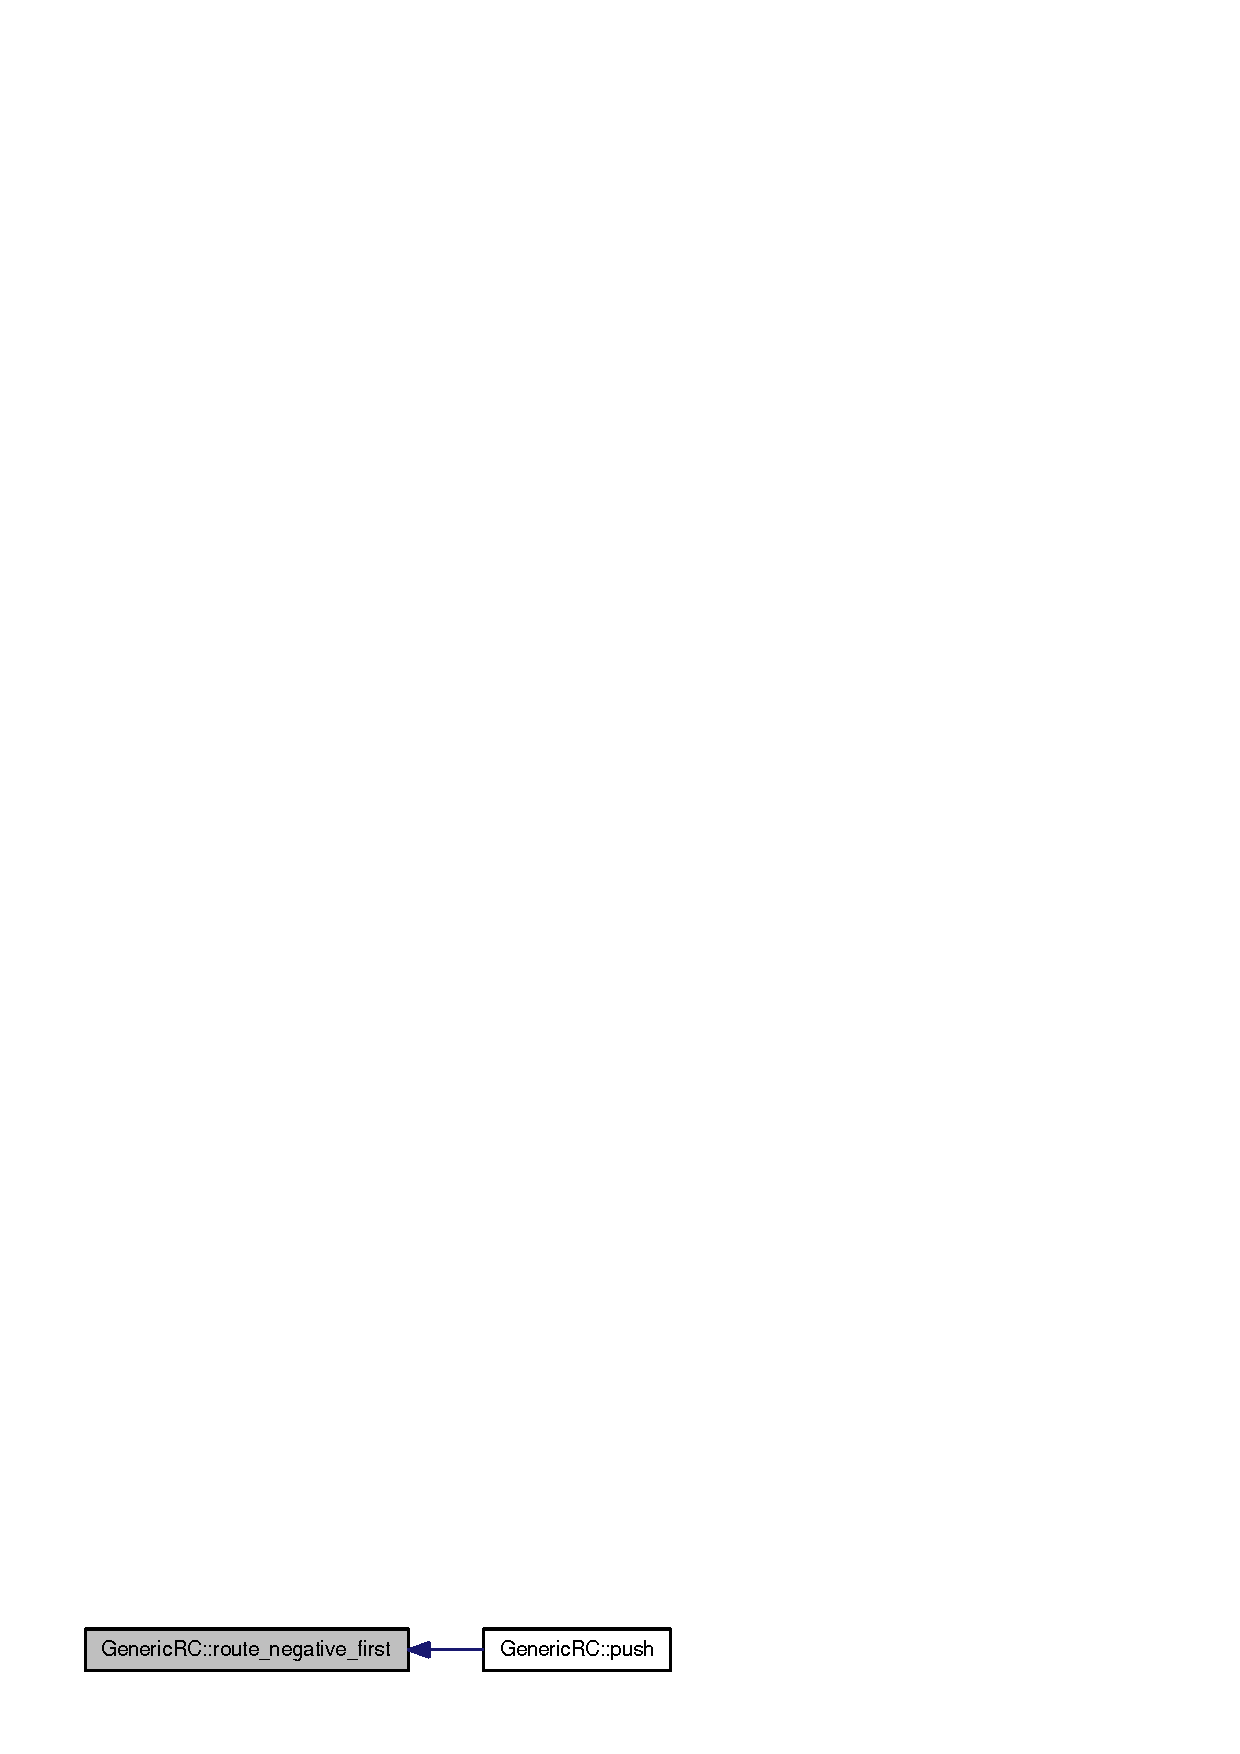
\includegraphics[width=163pt]{classGenericRC_45b503a8ac6becaa1660d2197ff126b2_icgraph}
\end{center}
\end{figure}
\index{GenericRC@{GenericRC}!route\_\-north\_\-last@{route\_\-north\_\-last}}
\index{route\_\-north\_\-last@{route\_\-north\_\-last}!GenericRC@{GenericRC}}
\subsubsection[{route\_\-north\_\-last}]{\setlength{\rightskip}{0pt plus 5cm}void GenericRC::route\_\-north\_\-last ({\bf HeadFlit} $\ast$ {\em hf})\hspace{0.3cm}{\tt  [private]}}\label{classGenericRC_eb0b5aafb2ca2c35e9e8949394c0f6c6}




Definition at line 196 of file genericRC.cc.

References \_\-DBG, HeadFlit::dst\_\-address, grid\_\-xloc, grid\_\-yloc, node\_\-ip, and possible\_\-out\_\-ports.

Referenced by push().

Here is the caller graph for this function:\nopagebreak
\begin{figure}[H]
\begin{center}
\leavevmode
\includegraphics[width=155pt]{classGenericRC_eb0b5aafb2ca2c35e9e8949394c0f6c6_icgraph}
\end{center}
\end{figure}
\index{GenericRC@{GenericRC}!route\_\-north\_\-last\_\-non\_\-minimal@{route\_\-north\_\-last\_\-non\_\-minimal}}
\index{route\_\-north\_\-last\_\-non\_\-minimal@{route\_\-north\_\-last\_\-non\_\-minimal}!GenericRC@{GenericRC}}
\subsubsection[{route\_\-north\_\-last\_\-non\_\-minimal}]{\setlength{\rightskip}{0pt plus 5cm}void GenericRC::route\_\-north\_\-last\_\-non\_\-minimal ({\bf HeadFlit} $\ast$ {\em hf})\hspace{0.3cm}{\tt  [private]}}\label{classGenericRC_10cdb1416ae7da4cc9430d9cfb3329b5}




Definition at line 276 of file genericRC.cc.

References \_\-DBG, HeadFlit::dst\_\-address, grid\_\-size, grid\_\-xloc, grid\_\-yloc, HeadFlit::inport, no\_\-nodes, node\_\-ip, possible\_\-out\_\-ports, and route\_\-x\_\-y().

Referenced by push().

Here is the caller graph for this function:\nopagebreak
\begin{figure}[H]
\begin{center}
\leavevmode
\includegraphics[width=185pt]{classGenericRC_10cdb1416ae7da4cc9430d9cfb3329b5_icgraph}
\end{center}
\end{figure}
\index{GenericRC@{GenericRC}!route\_\-odd\_\-even@{route\_\-odd\_\-even}}
\index{route\_\-odd\_\-even@{route\_\-odd\_\-even}!GenericRC@{GenericRC}}
\subsubsection[{route\_\-odd\_\-even}]{\setlength{\rightskip}{0pt plus 5cm}void GenericRC::route\_\-odd\_\-even ({\bf HeadFlit} $\ast$ {\em hf})\hspace{0.3cm}{\tt  [private]}}\label{classGenericRC_d526138b552d15f51d8683c71969182e}




Definition at line 360 of file genericRC.cc.

References \_\-DBG, HeadFlit::dst\_\-address, grid\_\-xloc, grid\_\-yloc, node\_\-ip, possible\_\-out\_\-ports, and HeadFlit::src\_\-address.

Referenced by push().

Here is the caller graph for this function:\nopagebreak
\begin{figure}[H]
\begin{center}
\leavevmode
\includegraphics[width=154pt]{classGenericRC_d526138b552d15f51d8683c71969182e_icgraph}
\end{center}
\end{figure}
\index{GenericRC@{GenericRC}!route\_\-west\_\-first@{route\_\-west\_\-first}}
\index{route\_\-west\_\-first@{route\_\-west\_\-first}!GenericRC@{GenericRC}}
\subsubsection[{route\_\-west\_\-first}]{\setlength{\rightskip}{0pt plus 5cm}void GenericRC::route\_\-west\_\-first ({\bf HeadFlit} $\ast$ {\em hf})\hspace{0.3cm}{\tt  [private]}}\label{classGenericRC_ff442fded7b3cda5205aa97e502fca2a}




Definition at line 129 of file genericRC.cc.

References \_\-DBG, HeadFlit::dst\_\-address, grid\_\-xloc, grid\_\-yloc, node\_\-ip, and possible\_\-out\_\-ports.

Referenced by push().

Here is the caller graph for this function:\nopagebreak
\begin{figure}[H]
\begin{center}
\leavevmode
\includegraphics[width=154pt]{classGenericRC_ff442fded7b3cda5205aa97e502fca2a_icgraph}
\end{center}
\end{figure}
\index{GenericRC@{GenericRC}!route\_\-x\_\-y@{route\_\-x\_\-y}}
\index{route\_\-x\_\-y@{route\_\-x\_\-y}!GenericRC@{GenericRC}}
\subsubsection[{route\_\-x\_\-y}]{\setlength{\rightskip}{0pt plus 5cm}{\bf uint} GenericRC::route\_\-x\_\-y ({\bf uint} {\em addr})\hspace{0.3cm}{\tt  [private]}}\label{classGenericRC_783f80da9e6aa41e6e91af1403db3270}




Definition at line 33 of file genericRC.cc.

References \_\-DBG, grid\_\-xloc, grid\_\-yloc, and node\_\-ip.

Referenced by push(), and route\_\-north\_\-last\_\-non\_\-minimal().

Here is the caller graph for this function:\nopagebreak
\begin{figure}[H]
\begin{center}
\leavevmode
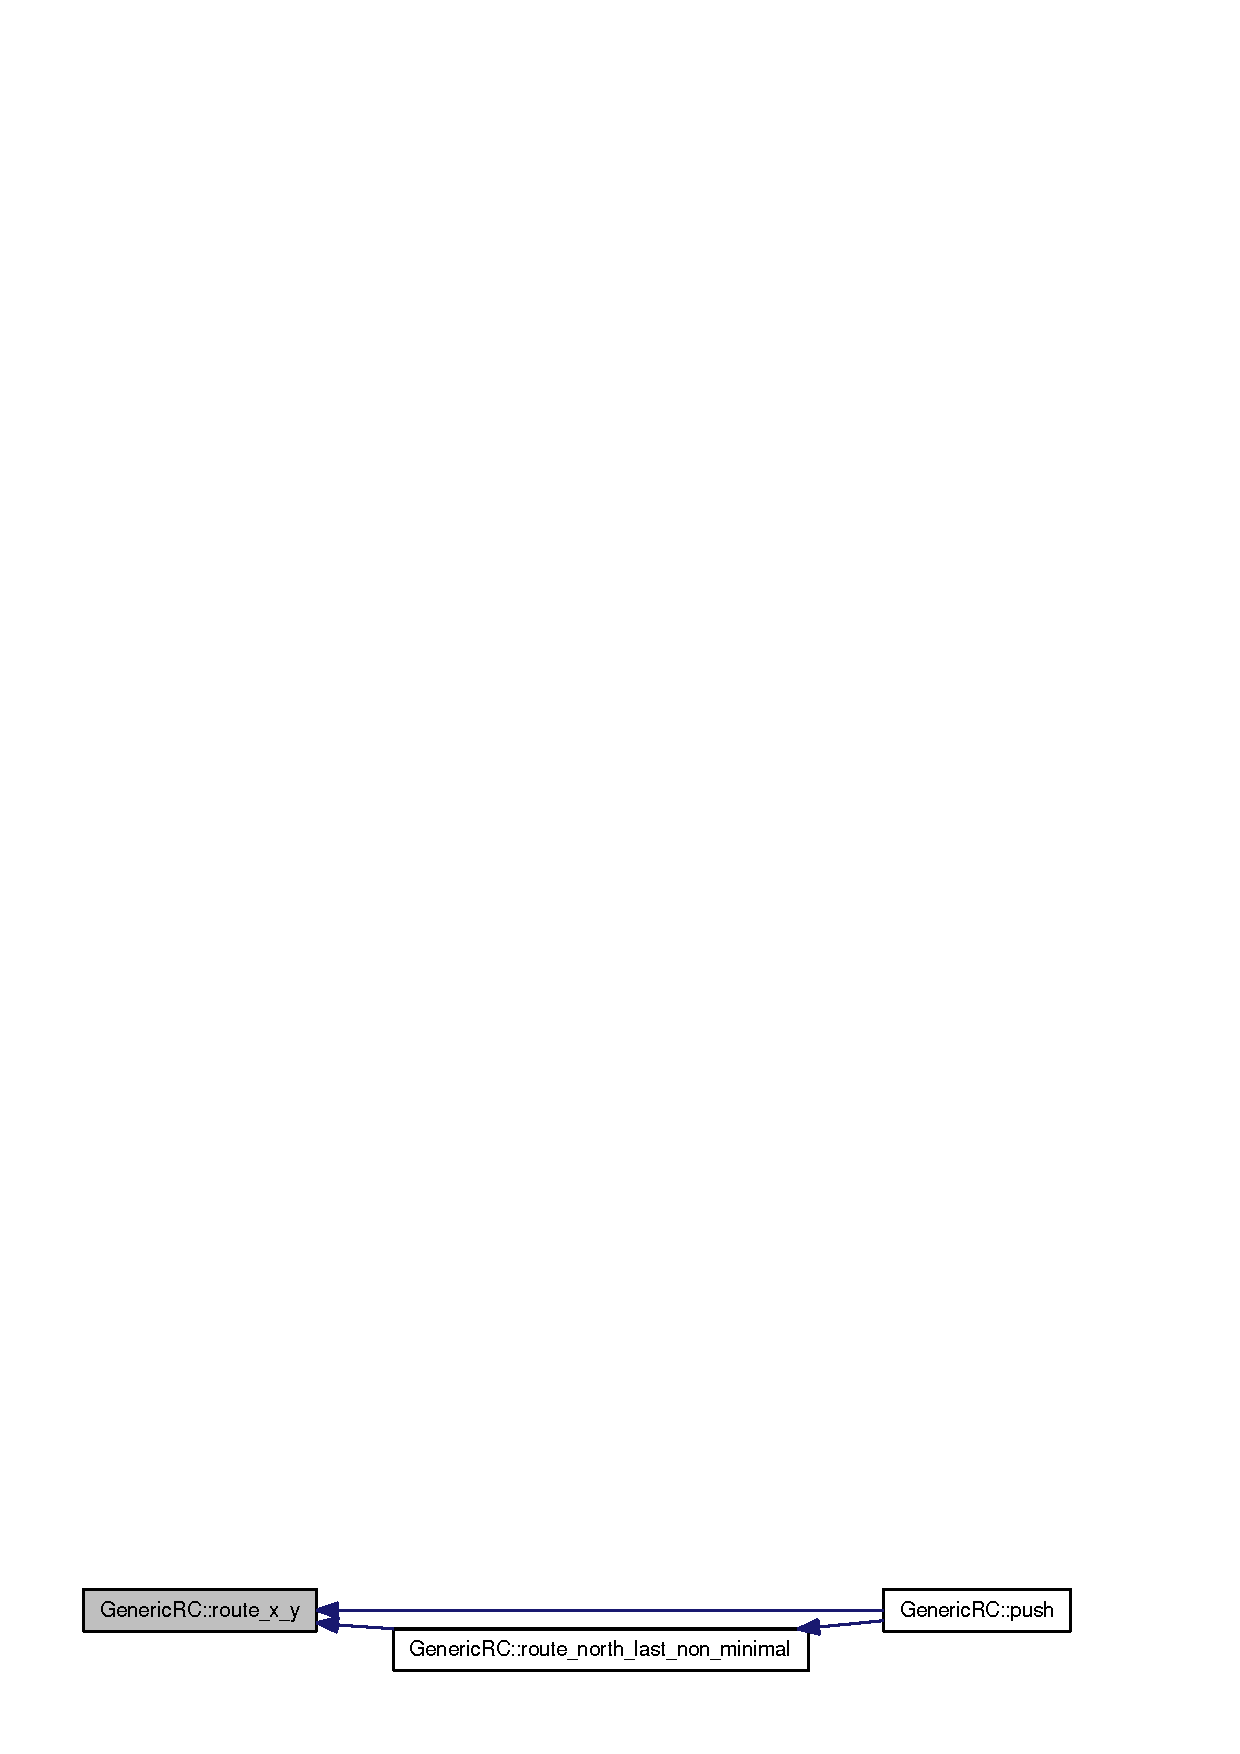
\includegraphics[width=259pt]{classGenericRC_783f80da9e6aa41e6e91af1403db3270_icgraph}
\end{center}
\end{figure}
\index{GenericRC@{GenericRC}!speculate\_\-channel@{speculate\_\-channel}}
\index{speculate\_\-channel@{speculate\_\-channel}!GenericRC@{GenericRC}}
\subsubsection[{speculate\_\-channel}]{\setlength{\rightskip}{0pt plus 5cm}{\bf uint} GenericRC::speculate\_\-channel ({\bf Flit} $\ast$ {\em f}, \/  {\bf uint} {\em ch})}\label{classGenericRC_2ebb540e1ca3fea96176908a9d21a3ad}


\index{GenericRC@{GenericRC}!speculate\_\-port@{speculate\_\-port}}
\index{speculate\_\-port@{speculate\_\-port}!GenericRC@{GenericRC}}
\subsubsection[{speculate\_\-port}]{\setlength{\rightskip}{0pt plus 5cm}{\bf uint} GenericRC::speculate\_\-port ({\bf Flit} $\ast$ {\em f}, \/  {\bf uint} {\em ch})}\label{classGenericRC_2607d570efd24c62511def45adceb067}


\index{GenericRC@{GenericRC}!toString@{toString}}
\index{toString@{toString}!GenericRC@{GenericRC}}
\subsubsection[{toString}]{\setlength{\rightskip}{0pt plus 5cm}string GenericRC::toString () const}\label{classGenericRC_214ef51af1dd900b41bb98b4826b5af4}




Definition at line 619 of file genericRC.cc.

References addresses.

\subsection{Member Data Documentation}
\index{GenericRC@{GenericRC}!address@{address}}
\index{address@{address}!GenericRC@{GenericRC}}
\subsubsection[{address}]{\setlength{\rightskip}{0pt plus 5cm}{\bf uint} {\bf GenericRC::address}}\label{classGenericRC_5a89c8b3e742b017f108ce1075422526}




Definition at line 56 of file genericRC.h.

Referenced by GenericRC().\index{GenericRC@{GenericRC}!addresses@{addresses}}
\index{addresses@{addresses}!GenericRC@{GenericRC}}
\subsubsection[{addresses}]{\setlength{\rightskip}{0pt plus 5cm}vector$<${\bf Address}$>$ {\bf GenericRC::addresses}\hspace{0.3cm}{\tt  [private]}}\label{classGenericRC_5e837760d9c3df33625c4f7c0d0a2c1f}




Definition at line 96 of file genericRC.h.

Referenced by get\_\-no\_\-channels(), get\_\-output\_\-port(), get\_\-virtual\_\-channel(), is\_\-empty(), no\_\-adaptive\_\-ports(), no\_\-adaptive\_\-vcs(), push(), resize(), and toString().\index{GenericRC@{GenericRC}!grid\_\-xloc@{grid\_\-xloc}}
\index{grid\_\-xloc@{grid\_\-xloc}!GenericRC@{GenericRC}}
\subsubsection[{grid\_\-xloc}]{\setlength{\rightskip}{0pt plus 5cm}vector$<$ {\bf uint} $>$ {\bf GenericRC::grid\_\-xloc}}\label{classGenericRC_2e2f02ddede7cfafca6073ee559663e2}




Definition at line 57 of file genericRC.h.

Referenced by route\_\-negative\_\-first(), route\_\-north\_\-last(), route\_\-north\_\-last\_\-non\_\-minimal(), route\_\-odd\_\-even(), route\_\-west\_\-first(), and route\_\-x\_\-y().\index{GenericRC@{GenericRC}!grid\_\-yloc@{grid\_\-yloc}}
\index{grid\_\-yloc@{grid\_\-yloc}!GenericRC@{GenericRC}}
\subsubsection[{grid\_\-yloc}]{\setlength{\rightskip}{0pt plus 5cm}vector$<$ {\bf uint} $>$ {\bf GenericRC::grid\_\-yloc}}\label{classGenericRC_89b5f8d2de4dc45ce64cbb0038ec0efa}




Definition at line 58 of file genericRC.h.

Referenced by route\_\-negative\_\-first(), route\_\-north\_\-last(), route\_\-north\_\-last\_\-non\_\-minimal(), route\_\-odd\_\-even(), route\_\-west\_\-first(), and route\_\-x\_\-y().\index{GenericRC@{GenericRC}!name@{name}}
\index{name@{name}!GenericRC@{GenericRC}}
\subsubsection[{name}]{\setlength{\rightskip}{0pt plus 5cm}string {\bf GenericRC::name}\hspace{0.3cm}{\tt  [private]}}\label{classGenericRC_c16b221c60eff6945123ab68d2d4fe22}




Definition at line 63 of file genericRC.h.

Referenced by GenericRC().\index{GenericRC@{GenericRC}!node\_\-ip@{node\_\-ip}}
\index{node\_\-ip@{node\_\-ip}!GenericRC@{GenericRC}}
\subsubsection[{node\_\-ip}]{\setlength{\rightskip}{0pt plus 5cm}{\bf uint} {\bf GenericRC::node\_\-ip}}\label{classGenericRC_f937d0d5d2df92a5be2641fb062f312e}




Definition at line 55 of file genericRC.h.

Referenced by GenericRC(), route\_\-negative\_\-first(), route\_\-north\_\-last(), route\_\-north\_\-last\_\-non\_\-minimal(), route\_\-odd\_\-even(), route\_\-west\_\-first(), and route\_\-x\_\-y().\index{GenericRC@{GenericRC}!possible\_\-out\_\-ports@{possible\_\-out\_\-ports}}
\index{possible\_\-out\_\-ports@{possible\_\-out\_\-ports}!GenericRC@{GenericRC}}
\subsubsection[{possible\_\-out\_\-ports}]{\setlength{\rightskip}{0pt plus 5cm}vector$<$ {\bf uint} $>$ {\bf GenericRC::possible\_\-out\_\-ports}\hspace{0.3cm}{\tt  [private]}}\label{classGenericRC_e743374f2f9663fefa0da8d25f584568}




Definition at line 71 of file genericRC.h.

Referenced by get\_\-output\_\-port(), push(), route\_\-negative\_\-first(), route\_\-north\_\-last(), route\_\-north\_\-last\_\-non\_\-minimal(), route\_\-odd\_\-even(), and route\_\-west\_\-first().\index{GenericRC@{GenericRC}!possible\_\-out\_\-vcs@{possible\_\-out\_\-vcs}}
\index{possible\_\-out\_\-vcs@{possible\_\-out\_\-vcs}!GenericRC@{GenericRC}}
\subsubsection[{possible\_\-out\_\-vcs}]{\setlength{\rightskip}{0pt plus 5cm}vector$<$ {\bf uint} $>$ {\bf GenericRC::possible\_\-out\_\-vcs}\hspace{0.3cm}{\tt  [private]}}\label{classGenericRC_b5f4f7b68f1c72e19e22220b293a399a}




Definition at line 72 of file genericRC.h.

Referenced by get\_\-virtual\_\-channel(), and push().\index{GenericRC@{GenericRC}!vcs@{vcs}}
\index{vcs@{vcs}!GenericRC@{GenericRC}}
\subsubsection[{vcs}]{\setlength{\rightskip}{0pt plus 5cm}{\bf uint} {\bf GenericRC::vcs}\hspace{0.3cm}{\tt  [private]}}\label{classGenericRC_d6ab0895975afb3d0607c1497840d651}




Definition at line 64 of file genericRC.h.

Referenced by push(), and resize().

The documentation for this class was generated from the following files:\begin{CompactItemize}
\item 
{\bf genericRC.h}\item 
{\bf genericRC.cc}\end{CompactItemize}
